\documentclass[12pt]{beamer} %Makes presentation

%\documentclass[handout]{beamer} %Makes Handouts
\usetheme{Singapore} %Gray with fade at top
\useoutertheme[subsection=false]{miniframes} %Supppress subsection in header
\useinnertheme{rectangles} %Itemize/Enumerate boxes
\usecolortheme{seagull} %Color theme
\usecolortheme{rose} %Inner color theme

\definecolor{light-gray}{gray}{0.75}
\definecolor{dark-gray}{gray}{0.55}
\setbeamercolor{item}{fg=light-gray}
\setbeamercolor{enumerate item}{fg=dark-gray}

\setbeamertemplate{navigation symbols}{}
\setbeamertemplate{mini frames}[default]
\setbeamercovered{dynamics}
\setbeamerfont*{title}{size=\Large,series=\bfseries}

%\setbeameroption{notes on second screen} %Dual-Screen Notes
%\setbeameroption{show only notes} %Notes Output

\setbeamertemplate{frametitle}{\vspace{.5em}\bfseries\insertframetitle}
\newcommand{\heading}[1]{\noindent \textbf{#1}\\ \vspace{1em}}

\usepackage{bbding,color,multirow,times,ccaption,tabularx,graphicx,verbatim,booktabs,fixltx2e}
\usepackage{colortbl} %Table overlays
\usepackage[english]{babel}
\usepackage[latin1]{inputenc}
\usepackage[T1]{fontenc}

%\author[]{Thomas J. Leeper}
\institute[]{
  \inst{}%
  Department of Political Science and Government\\Aarhus University
}


\title{The Judiciary}

\date[]{October 9, 2014}

\begin{document}

\frame{\titlepage}

\frame{\tableofcontents}

\section{Presidency (cont.)}
\frame{\tableofcontents[currentsection]}


\frame{
	\frametitle{\textit{Cheney's Law}}
	\begin{itemize}\itemsep2em
		\item Frontline episode about Bush administration efforts to increase executive power in the immediate post-September 11th era
		\item \url{http://video.pbs.org/video/1082073775/}
		\item We'll just watch the first 15 minutes or so
	\end{itemize}
}


\frame{
\frametitle{Think--Pair--Share}	
	\begin{itemize}\itemsep2em
        \item Take 45 seconds to think about the following:
            \begin{itemize}
            \item What keeps the President from asserting complete unilateral authority?
            \end{itemize}
		\item Discuss for 90 seconds with the person sitting next to you
		\item Share with the class
	\end{itemize}
	
}

\section{The Judiciary}
\frame{\tableofcontents[currentsection]}

\frame{
	\frametitle{Common Law}
	\begin{itemize}\itemsep1em
		\item U.S. legal system is based in English Common Law
		\item Most states and the federal courts enforce pre-1776 British laws and precedent
		\item \textit{Stare decisis}: precedent whereby judicial decisions have the force of law
		\item Modifications noted in Constitution and Bill of Rights, e.g.,
			\begin{itemize}
				\item No Bills of Attainder
				\item 1st Amendments prohibits libel cases
				\item No \textit{ex post facto} laws
				\item Trial by jury
			\end{itemize}
	\end{itemize}
}

\frame{
	\frametitle{The Judiciary}
	\begin{itemize}\itemsep2em
		\item Constitution was an extremely minimal framework
		\item Recall the \textit{Articles} gave Congress judicial authority
		\item Court gets to regulate itself
		\item Congress can create lower courts
	\end{itemize}	
}

\frame{
	\frametitle{The Supreme Court (SCOTUS)}
	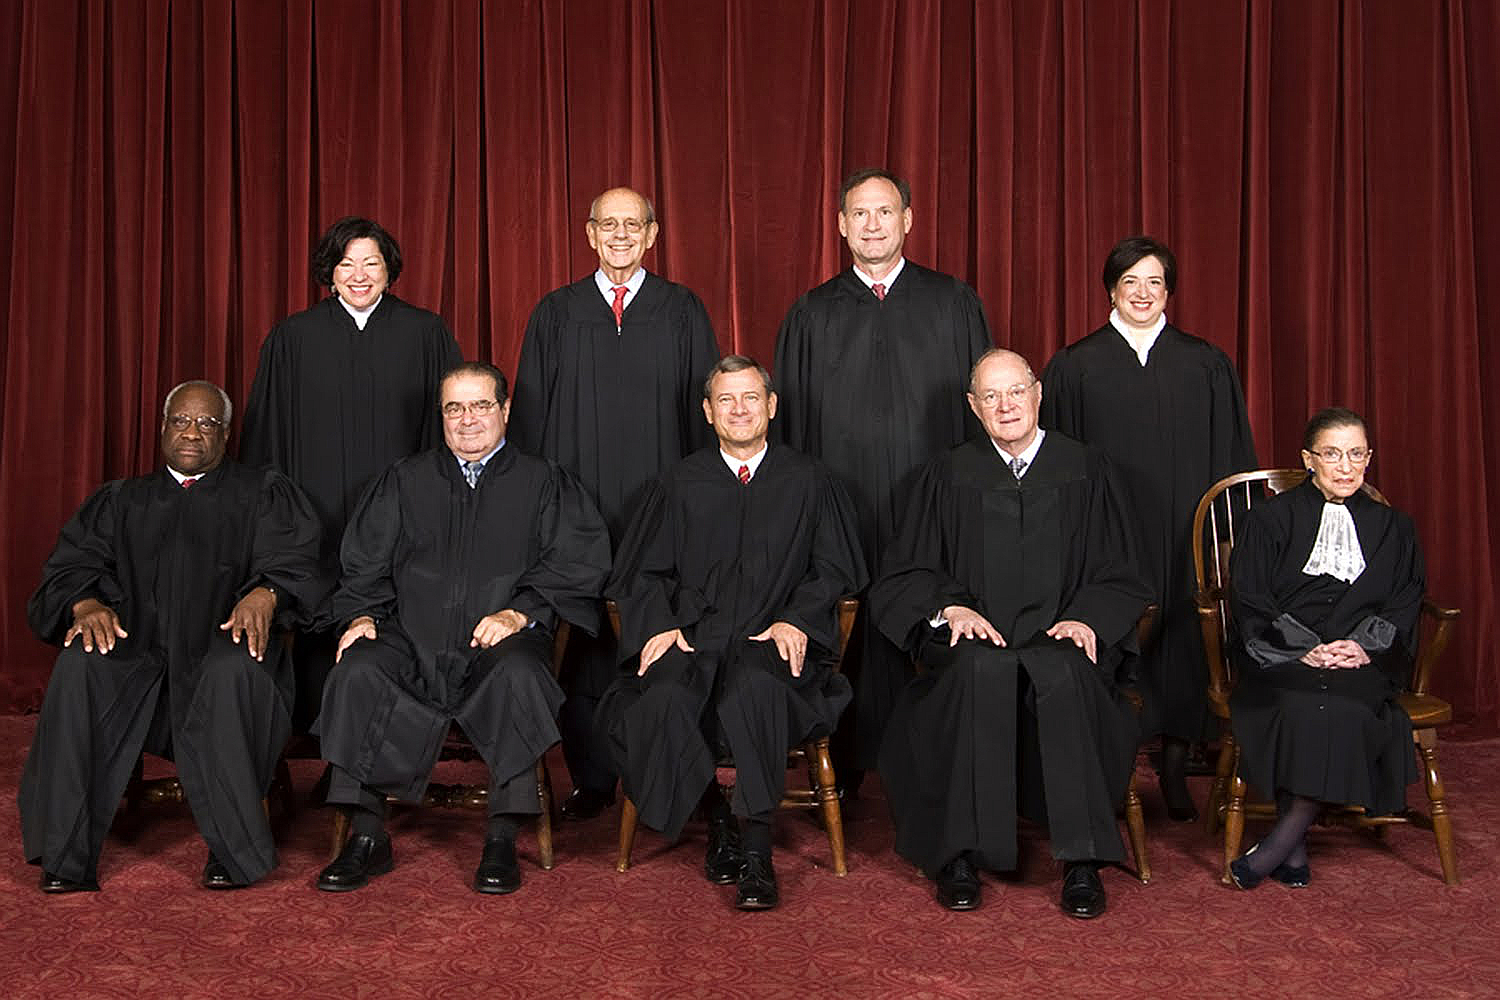
\includegraphics[width=\textwidth]{images/SCOTUS2010.png}
}

\frame{
	\frametitle{The Supreme Court (SCOTUS)}
	\begin{itemize}\itemsep1em
		\item Nine justices (by convention)
		\item Meet annually
		\item Appointed by President, approved by Senate
		\item Members serve lifetime terms
		\item Court of last resort
		\item Jurisdication
			\begin{itemize}
				\item Original (defined by Constitution)
				\item Appellate (defined by Congress)
			\end{itemize}
	\end{itemize}	
}

\frame{
	\frametitle{Lower Federal Courts}
	\begin{itemize}\itemsep1em
		\item 94 U.S. District Courts
		\item 12 U.S. Court of Appeals circuits
		\item Other ``Courts of Special Jurisdiction''
			\begin{itemize}
				\item E.g., Court of Federal Claims
			\end{itemize}
		\item Military Courts
	\end{itemize}	
}

\frame{
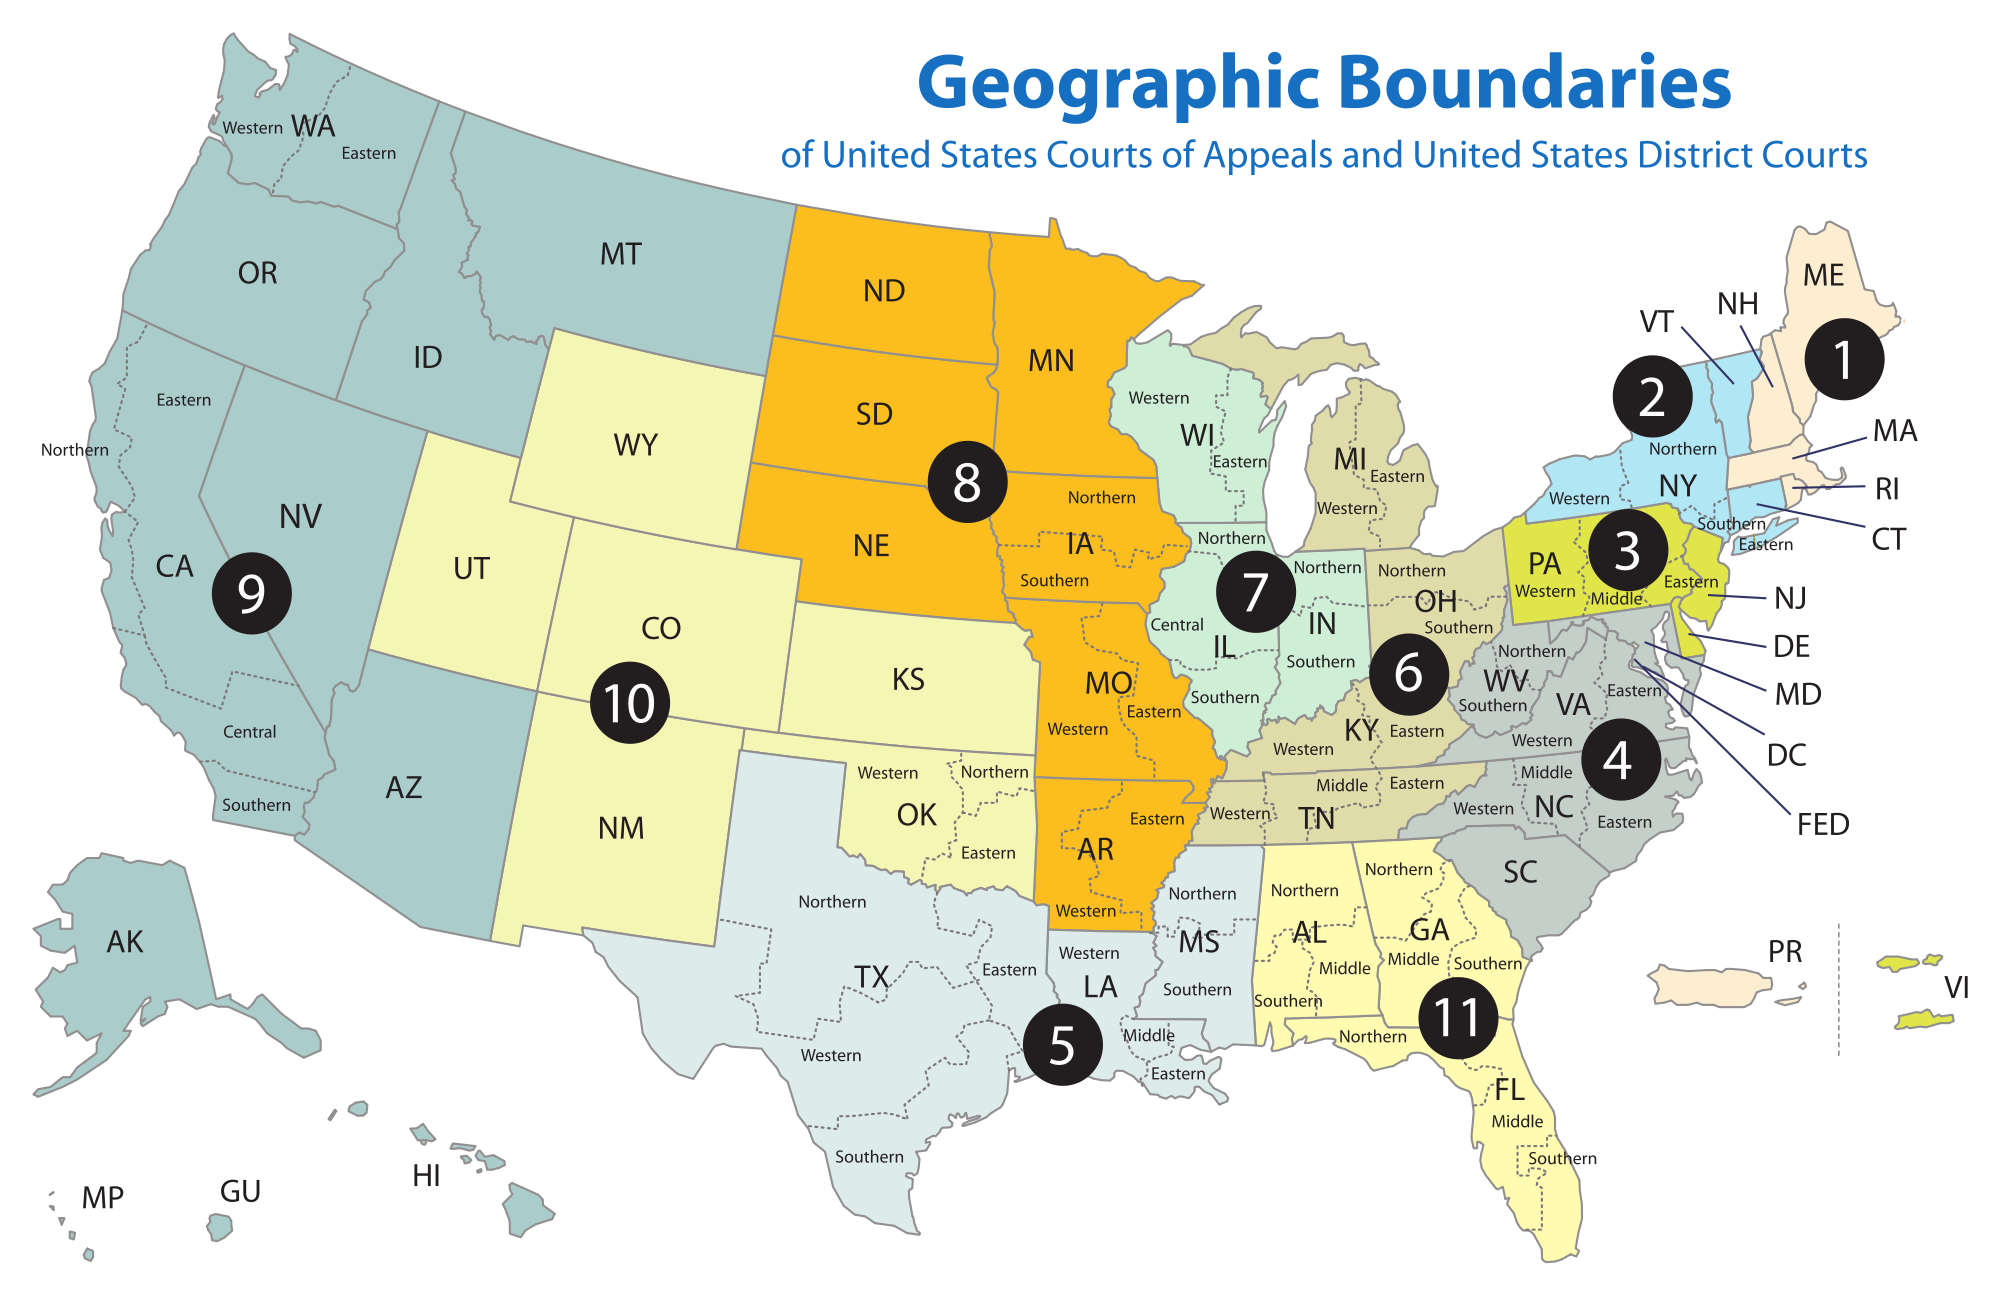
\includegraphics[width=\textwidth]{images/USCourtDistricts.png}	
}


\frame{
	\frametitle{State Courts}
	\begin{itemize}\itemsep1em
		\item Regulated by individual states
		\item 48 states have Supreme Court
			\begin{itemize}
				\item OK and TX have separate criminal and civil superior courts
				\item Justices typically serve fixed, renewable terms
				\item Four states have life terms
			\end{itemize}
		\item State district courts
		\item County/local courts
		\item Judges obtain office through either election or appointment
	\end{itemize}	
}

\frame{
	\frametitle{Federalism}
	\begin{itemize}\itemsep1em
		\item State courts are not subordinate to federal courts
		\item Federal laws overrule state laws when in conflict
		\item Federal appeals courts cannot review laws addressing only \textit{state} laws
		\item Appeals from state supreme courts can be taken to the Supreme Court if a federal law or constitutional issue is at-stake
	\end{itemize}	
}


\frame{
	\frametitle{Interbranch Relations}
	\begin{itemize}\itemsep1em
		\item President appoints federal judges
		\item Congress can impeach judges/justices
		\item Judiciary has no enforcement or revenue-raising powers
		\item SCOTUS can declare laws and executive actions unconstitutional
		\begin{itemize}
			\item Only when case exists
		\end{itemize}
	\end{itemize}	
}

\frame{
	\frametitle{Route to Supreme Court Review}
	\begin{itemize}\itemsep1em
		\item No one has a right to a SCOTUS appeal hearing
		\item SCOTUS grants \textit{certiorari} on its own discretion
		\item Without cert., lower court rulings stand
		\item Caseload: about 10,000 cases/year
		\item Cert. granted: 80--90
		\item Cert. guarantees nothing
	\end{itemize}	
}

\frame{
	\frametitle{When Does SCOTUS Grant cert.?}
	\begin{itemize}\itemsep1em
		\item Litigant appeals lower court ruling
		\item Reasons aren't always clear
		\begin{itemize}
			\item Public opinion?
			\item Interbranch relations?
			\item ``Split circuits''
		\end{itemize}
		\item Law clerks recommend cases to justices
		\item Litigants can repeatedly request cert.
		\item Requires four justices
		\begin{itemize}
			\item Decisions require majority rule
		\end{itemize}
	\end{itemize}	
}

\frame{
	\frametitle{How does SCOTUS decide cases?}
	\begin{itemize}\itemsep1em
		\item Written petitions from litigants
		\item Amici curae (friend of the court) briefs
		\item Oral arguments
		\item Secret meeting of justices
		\item Writing of opinions
			\begin{itemize}
				\item Opinion of the court
				\item Concurring opinions
				\item Dissenting opinions
			\end{itemize}
		\item Presentation of ruling
	\end{itemize}	
}

\frame{
	\frametitle{How does SCOTUS decide cases?}
	\begin{itemize}\itemsep1em
		\item Wording of the Constitution
		\item<2-> \textit{Meaning} of the Constitution
		\begin{itemize}
			\item<2-> Originalism
			\item<2-> ``Living constitution''
		\end{itemize}
		\item<3-> Laws
		\item<4-> Legal precedent
		\item<5-> Legal arguments
		\item<6-> Ideology
		\item<7-> Interbranch relations
		\item<8-> Public legitimacy
	\end{itemize}	
}


\frame{\frametitle{Questions about SCOTUS?}}
	
	
\frame{
	\frametitle{Activity: Important Cases}
	\begin{itemize}\itemsep1em
		\item List of important SCOTUS cases
		\item Research the cases online
		\item Share with the class and discuss
	\end{itemize}
}


\frame{
	\frametitle{Example: \textit{Marbury v. Madison} (1803)}
	\begin{itemize}\itemsep1em
		\item Marbury feels he deserves a public commission
		\item He challenges the government (Madison) at Supreme Court
		\item SCOTUS sides with Marbury on substance
		\item But! SCOTUS denies Marbury on grounds that Congress could not grant SCOTUS original jurisdiction in this case
		\item Conclusion: SCOTUS asserts right of judicial review
	\end{itemize}
}


\frame{\frametitle{Open Discussion}}


\section{Preview of Next Time}
\frame{\tableofcontents[currentsection]}

\frame{
	\frametitle{Next session's agenda}
	\begin{itemize}\itemsep2em
        \item No class next week
		\item State and local politics
		\begin{itemize}
			\item Differences between states
			\item Electoral politics
		\end{itemize}
	\end{itemize}
}

\frame{
	\frametitle{Sign-up for Presentations}
}

\appendix
\frame{}

\end{document}
